\documentclass[USenglish,aspectratio=169]{beamer} % either 'ngerman' or 'USenglish'

\usetheme{metropolis}

% general
% \usepackage{babel}
% \usepackage{csquotes}
\usepackage{xcolor}
\usepackage{colortbl}
\usepackage{hyperref}
\usepackage[
  backend=biber,
  url=false,
  style=ieee,
  citestyle=ieee
]{biblatex}
\addbibresource{references.bib}

\usepackage{soul}
% tables
\usepackage{tabularx}
\usepackage{array}
\usepackage{multirow}
\usepackage{multicol}
\usepackage{booktabs}
\usepackage{makecell} % for line breaks in table cells

% math
\usepackage{amsmath}
\usepackage{amsfonts}
\usepackage{amssymb}
\usepackage{amsthm}
\usepackage{centernot}
\usepackage{bm}

% figures
\usepackage{graphicx}
\usepackage{tikz}
\usepackage{pgfplots} 
\usepackage{pgfplotstable}
\usepackage{filecontents}
\usepgfplotslibrary{colorbrewer}
\pgfplotsset{compat=1.16, cycle list/Set1-8} 

% \usepackage{appendixnumberbeamer} % might cause arithmetic overflow error!
\usepackage{glossaries}
\usepackage{adjustbox}

\usepackage{listings}
\lstset{
    escapeinside={*@}{@*},
    showspaces=false,
    showstringspaces=false,
    showtabs=false
    xleftmargin=1pt,
    xrightmargin=1pt,
    aboveskip=1pt,
    belowskip=1pt,
    columns=fullflexible
}
\setlength\fboxsep{1pt}

\title{Undo and Redo Support for Replicated Registers}
\subtitle{PaPoC '24, Athens}
\author{Leo Stewen and Martin Kleppmann}
\date{April, 2024}

\graphicspath{{figures/}{../figures/}}
\hypersetup{
  pdftitle=\title,
  pdfauthor=\author,
  bookmarksopen=true,
  hidelinks,
}

\definecolor{opset1}{rgb}{0, 0.5, 1}
\definecolor{opset2}{rgb}{0.5, 0, 1}
\definecolor{opset3}{rgb}{0, 0.5, 0}
\definecolor{opset4}{rgb}{1, 0, 0}
\metroset{numbering=fraction,progressbar=frametitle,block=fill}
\setbeamertemplate{section in toc}[sections numbered]
\def\black{black}
\def\green{green!70!black}
\def\red{red}
\def\maxheightshare{0.8}

\usetikzlibrary{
  automata,
  positioning,
  arrows, arrows.meta,
  calc, backgrounds, quotes,
  pgfplots.statistics, pgfplots.colorbrewer,
  patterns
}

\tikzset{
  op/.style={
    font=\scriptsize,
    state,
    minimum size=44.0pt,
    fill=white,
  },
  head/.style={
    op,
    accepting,
  },
  edge/.style={
    ->,
    >={Stealth[round]},
  },
  pred/.style={
    edge,
  },
  anchorref/.style={
    edge,
    blue,
    densely dashed,
  },
  stepmarker/.style={
    font=\footnotesize,
    fill=black!10,
  },
  stepline/.style={
    edge,
    black!70,
    dotted,
    semithick,
    -,
  },
}

\newcommand*{\fullref}[1]{\hyperref[{#1}]{\autoref*{#1}}}
\newcommand{\op}[3][op]{$\mathit{#1}_{#2}^{#3}$} % with op kind
\newcommand{\opid}[2]{$\mathit{_{#1}^{#2}}$}
\newcommand{\setop}[4][set]{$\mathit{#1_{#2}^{#3}(#4)}$}
\newcommand{\delop}[3][del]{$\mathit{#1_{#2}^{#3}()}$}
\newcommand{\undop}[5][undo]{$\mathit{#1_{#2}^{#3}(_{#4}^{#5})}$}
\newcommand{\redop}[5][redo]{$\mathit{#1_{#2}^{#3}(_{#4}^{#5})}$}
\newcommand{\restop}[5][rest]{$\mathit{#1_{#2}^{#3}(_{#4}^{#5})}$}
\def\setabbr{s}
\def\restabbr{rs}
\newcommand{\setopkind}{\textit{SetOp}}
\newcommand{\restopkind}{\textit{RestoreOp}}
\newcommand{\opidtrace}{\textit{OpIdTrace}}

\newcounter{figcase}

%% CONTENT

\begin{document}

\begin{frame}
\maketitle
\end{frame}

% \begin{frame}{Contents}
% \tableofcontents
% \end{frame}

\section{Part I: Undo Semantics in a Collaborative Setting}

\begin{frame}[fragile,plain]
  \begin{figure}
  \centering
  \begin{tikzpicture}[node distance=0.50cm]
    \coordinate (c0) at (0,0);

    \tikzset{
      canvas/.style={
        rectangle,
        draw,
        anchor = west,
        inner sep = 4pt,
      },
      rect/.style={
        rectangle,
        minimum width = 1.2cm, 
        minimum height = 0.5cm,
        inner sep = 0.1cm,
        text = white,
        fill = #1,
      },
      optrans/.style={
        <-,bend right=90,>={Stealth[round]},
        swap,
        black!70,
      },
      next/.style={
        <-,
        >={Stealth[round]},
      },
      caselabel/.style={
        rectangle,
        minimum width = 238.5pt,
        % just for left align of text
        text width=260pt,
      },
    }

    \def\black{black}
    \def\green{green!70!black}
    \def\red{red}
    \def\upperoffset{22pt}
    \def\casemargin{22pt}
    \def\caselabeldist{1pt}

    % two registers, global undo

    \onslide<3->{
    \node[
      canvas,
    ] (a1) at (c0) {
      \begin{tikzpicture}[node distance=3pt]
        \node[
            rect=\black,
          ] (r1) at (0,0) {\vphantom{bg}black};
        \node[
            rect=\black,
            below = of r1,
          ] (r2) {\vphantom{bg}black};
      \end{tikzpicture}
    };
    }

    \onslide<4->{
    \node[
      canvas,
      right = of a1,
    ] (a2) {
      \begin{tikzpicture}[node distance=3pt]
        \node[
            rect=\red,
          ] (r1) at (0,0) {\vphantom{bg}red};
        \node[
            rect=\black,
            below = of r1,
          ] (r2) {\vphantom{bg}black};
      \end{tikzpicture}
    } edge [next] (a1);
    }

    \onslide<5->{
    \node[
      canvas,
      right = of a2,
    ] (a3) {
      \begin{tikzpicture}[node distance=3pt]
        \node[
            rect=\red,
          ] (r1) at (0,0) {\vphantom{bg}red};
        \node[
            rect=\green,
            below = of r1,
          ] (r2) {\vphantom{bg}green};
      \end{tikzpicture}
    } edge [next] (a2);
    }

    \onslide<6->{
    \node[
      canvas,
      right = of a3,
    ] (a4) {
      \begin{tikzpicture}[node distance=3pt]
        \node[
            rect=\red,
          ] (r1) at (0,0) {\vphantom{bg}red};
        \node[
            rect=\black,
            below = of r1,
          ] (r2) {\vphantom{bg}black};
      \end{tikzpicture}
    } edge [next] (a3);
    }

    \onslide<7->{
    \node[
      canvas,
      right = of a4,
    ] (a5) {
      \begin{tikzpicture}[node distance=3pt]
        \node[
            rect=\red,
          ] (r1) at (0,0) {\vphantom{bg}red};
        \node[
            rect=\green,
            below = of r1,
          ] (r2) {\vphantom{bg}green};
      \end{tikzpicture}
    } edge [next] (a4);
    }

    % two registers, local undo

    \onslide<9->{
    \node[
      canvas,
      below=\casemargin of a1,
    ] (b1) {
      \begin{tikzpicture}[node distance=3pt]
        \node[
            rect=\black,
          ] (r1) at (0,0) {\vphantom{bg}black};
        \node[
            rect=\black,
            below = of r1,
          ] (r2) {\vphantom{bg}black};
      \end{tikzpicture}
    };
    }

    \onslide<9->{
    \node[
      canvas,
      right = of b1,
    ] (b2) {
      \begin{tikzpicture}[node distance=3pt]
        \node[
            rect=\red,
          ] (r1) at (0,0) {\vphantom{bg}red};
        \node[
            rect=\black,
            below = of r1,
          ] (r2) {\vphantom{bg}black};
      \end{tikzpicture}
    } edge [next] (b1);
    }

    \onslide<9->{
    \node[
      canvas,
      right = of b2,
    ] (b3) {
      \begin{tikzpicture}[node distance=3pt]
        \node[
            rect=\red,
          ] (r1) at (0,0) {\vphantom{bg}red};
        \node[
            rect=\green,
            below = of r1,
          ] (r2) {\vphantom{bg}green};
      \end{tikzpicture}
    } edge [next] (b2);
    }

    \onslide<10->{
    \node[
      canvas,
      right = of b3,
    ] (b4) {
      \begin{tikzpicture}[node distance=3pt]
        \node[
            rect=\black,
          ] (r1) at (0,0) {\vphantom{bg}black};
        \node[
            rect=\green,
            below = of r1,
          ] (r2) {\vphantom{bg}green};
      \end{tikzpicture}
    } edge [next] (b3);
    }

    \onslide<11->{
    \node[
      canvas,
      right = of b4,
    ] (b5) {
      \begin{tikzpicture}[node distance=3pt]
        \node[
            rect=\red,
          ] (r1) at (0,0) {\vphantom{bg}red};
        \node[
            rect=\green,
            below = of r1,
          ] (r2) {\vphantom{bg}green};
      \end{tikzpicture}
    } edge [next] (b4);
    }

    % ops

    \draw (a2.north)+(-0.2cm,+\upperoffset) edge ["A set",optrans] ($(a1.north)+(0,+\upperoffset)$);
    \draw (a3.north)+(-0.2cm,+\upperoffset) edge ["B set",optrans] ($(a2.north)+(0,+\upperoffset)$);
    \draw (a4.north)+(-0.2cm,+\upperoffset) edge ["A undo",optrans] ($(a3.north)+(0,+\upperoffset)$);
    \draw (a5.north)+(-0.2cm,+\upperoffset) edge ["A redo",optrans] ($(a4.north)+(0,+\upperoffset)$);

    % case labels

    \onslide< 2->{
    \node[caselabel,above=\caselabeldist of a3] {
      1) Global undo
    };
    }

    \onslide< 8->{
    \node[caselabel,above=\caselabeldist of b3] {
      2) Local undo
    };
    }

  \end{tikzpicture}
  \caption{
    Users $A$ and $B$ collaboratively edit \emph{\textbf{two} registers}.
  }\label{fig:semantics-two-registers}
  \end{figure}

\end{frame}

\begin{frame}[fragile,plain]
  \begin{figure}
  \centering
  \begin{tikzpicture}[node distance=0.50cm]
    \coordinate (c0) at (0,0);

    \tikzset{
      canvas/.style={
        rectangle,
        draw,
        anchor = west,
        inner sep = 4pt,
      },
      rect/.style={
        rectangle,
        minimum width = 1.2cm, 
        minimum height = 0.5cm,
        inner sep = 0.1cm,
        text = white,
        fill = #1,
      },
      optrans/.style={
        <-,bend right=90,>={Stealth[round]},
        swap,
        black!70,
      },
      next/.style={
        <-,
        >={Stealth[round]},
      },
      caselabel/.style={
        rectangle,
        minimum width = 238.5pt,
        % just for left align of text
        text width=260pt,
      },
    }

    \def\black{black}
    \def\green{green!70!black}
    \def\red{red}
    \def\upperoffset{22pt}
    \def\casemargin{22pt}
    \def\caselabeldist{1pt}

    % one register, global undo

    \onslide< 1->{
    \node[
      canvas,
    ] (c1) at (c0) {
      \begin{tikzpicture}[node distance=3pt]
        \node[
            rect=\black,
          ] (r1) at (0,0) {\vphantom{bg}black};
      \end{tikzpicture}
    };
    }

    \onslide< 2->{
    \node[
      canvas,
      right = of c1,
    ] (c2) {
      \begin{tikzpicture}[node distance=3pt]
        \node[
            rect=\red,
          ] (r1) at (0,0) {\vphantom{bg}red};
      \end{tikzpicture}
    } edge [next] (c1);
    }

    \onslide< 3->{
    \node[
      canvas,
      right = of c2,
    ] (c3) {
      \begin{tikzpicture}[node distance=3pt]
        \node[
            rect=\green,
          ] (r1) at (0,0) {\vphantom{bg}green};
      \end{tikzpicture}
    } edge [next] (c2);
    }

    \onslide< 4->{
    \node[
      canvas,
      right = of c3,
    ] (c4) {
      \begin{tikzpicture}[node distance=3pt]
        \node[
            rect=\red,
          ] (r1) at (0,0) {\vphantom{bg}red};
      \end{tikzpicture}
    } edge [next] (c3);
    }

    \onslide< 5->{
    \node[
      canvas,
      right = of c4,
    ] (c5) {
      \begin{tikzpicture}[node distance=3pt]
        \node[
            rect=\green,
          ] (r1) at (0,0) {\vphantom{bg}green};
      \end{tikzpicture}
    } edge [next] (c4);
    }

    % one register, local undo

    \onslide< 7->{
    \node[
      canvas,
      below=\casemargin of c1,
    ] (d1) {
      \begin{tikzpicture}[node distance=3pt]
        \node[
            rect=\black,
          ] (r1) at (0,0) {\vphantom{bg}black};
      \end{tikzpicture}
    };
    }

    \onslide< 7->{
    \node[
      canvas,
      right = of d1,
    ] (d2) {
      \begin{tikzpicture}[node distance=3pt]
        \node[
            rect=\red,
          ] (r1) at (0,0) {\vphantom{bg}red};
      \end{tikzpicture}
    } edge [next] (d1);
    }

    \onslide< 7->{
    \node[
      canvas,
      right = of d2,
    ] (d3) {
      \begin{tikzpicture}[node distance=3pt]
        \node[
            rect=\green,
          ] (r1) at (0,0) {\vphantom{bg}green};
      \end{tikzpicture}
    } edge [next] (d2);
    }

    \onslide< 8->{
    \node[
      canvas,
      right = of d3,
    ] (d4) {
      \begin{tikzpicture}[node distance=3pt]
        \node[
            rect=\black,
          ] (r1) at (0,0) {\vphantom{bg}black};
      \end{tikzpicture}
    } edge [next] (d3);
    }

    \onslide< 9->{
    \node[
      canvas,
      right = of d4,
    ] (d5) {
      \begin{tikzpicture}[node distance=3pt]
        \node[
            rect=\green,
          ] (r1) at (0,0) {\vphantom{bg}green};
      \end{tikzpicture}
    } edge [next] (d4);
    }

    % one register, remote op blocks undo

    \onslide<11->{
    \node[
      canvas,
      below=\casemargin of d1,
    ] (e1) {
      \begin{tikzpicture}[node distance=3pt]
        \node[
            rect=\black,
          ] (r1) at (0,0) {\vphantom{bg}black};
      \end{tikzpicture}
    };
    }

    \onslide<11->{
    \node[
      canvas,
      right = of e1,
    ] (e2) {
      \begin{tikzpicture}[node distance=3pt]
        \node[
            rect=\red,
          ] (r1) at (0,0) {\vphantom{bg}red};
      \end{tikzpicture}
    } edge [next] (e1);
    }

    \onslide<11->{
    \node[
      canvas,
      right = of e2,
    ] (e3) {
      \begin{tikzpicture}[node distance=3pt]
        \node[
            rect=\green,
          ] (r1) at (0,0) {\vphantom{bg}green};
      \end{tikzpicture}
    } edge [next] (e2);
    }

    \onslide<12->{
    \node[
      canvas,
      right = of e3,
    ] (e4) {
      \begin{tikzpicture}[node distance=3pt]
        \node[
            rect=\green,
          ] (r1) at (0,0) {\vphantom{bg}green};
      \end{tikzpicture}
    } edge [next] (e3);
    }

    \onslide<13->{
    \node[
      canvas,
      right = of e4,
    ] (e5) {
      \begin{tikzpicture}[node distance=3pt]
        \node[
            rect=\green,
          ] (r1) at (0,0) {\vphantom{bg}green};
      \end{tikzpicture}
    } edge [next] (e4);
    }

    % ops

    \draw (c2.north)+(-0.2cm,+\upperoffset) edge ["A set",optrans] ($(c1.north)+(0,+\upperoffset)$);
    \draw (c3.north)+(-0.2cm,+\upperoffset) edge ["B set",optrans] ($(c2.north)+(0,+\upperoffset)$);
    \draw (c4.north)+(-0.2cm,+\upperoffset) edge ["A undo",optrans] ($(c3.north)+(0,+\upperoffset)$);
    \draw (c5.north)+(-0.2cm,+\upperoffset) edge ["A redo",optrans] ($(c4.north)+(0,+\upperoffset)$);

    % case labels

    \onslide< 1->{
    \node[caselabel,above=\caselabeldist of c3] {
      3) Global undo
    };
    }

    \onslide< 6->{
    \node[caselabel,above=\caselabeldist of d3] {
      4) Local undo
    };
    }

    \onslide<10->{
    \node[caselabel,above=\caselabeldist of e3] {
      5) Remote operation blocks undo
    };
    }

    \onslide<14->{
    \def\offset{1.5cm}
    \node[right=\offset of d5,anchor=center] (lundo)
    {
\includegraphics[height=60px]{local_undo_users.png}}; 

    \node[right=\offset of e5,anchor=center] (bundo)
    {\includegraphics[height=25px]{miro.png}}; 
    }

  \end{tikzpicture}
  \caption{
    Users $A$ and $B$ collaboratively edit \emph{\textbf{one} register}.
  }\label{fig:semantics-single-register}
  \end{figure}

\end{frame}

\section{Part II: An Algorithm for (Local) Undo}

\newcommand{\cbox}[1]{\colorbox{#1}{\phantom{R}}}

\newcommand{\mvr}[1]{
  \begin{tikzpicture}[]
    \tikzset{
      sitem/.style={
        minimum width=40px,
        minimum height=17px,
        rectangle,
        font=\scriptsize,
      }
    }
    \node[font=\Large,minimum width=40px] (empty) at (0,0.46) {$\bot$};
    \foreach \x [count=\i] in #1 {
      \ifnum \i=1
        \node[sitem,draw,fill=gray!20] (s\i) at (0,0.59*\i) {\x};
      \else
        \node[sitem,draw,fill=white] (s\i) at (0,0.59*\i) {\x};
      \fi
    }
  \end{tikzpicture}
}
\newcommand{\stack}[1]{
  \begin{tikzpicture}[]
    \tikzset{
      sitem/.style={
        minimum width=40px,
        minimum height=17px,
        rectangle,
        font=\scriptsize,
      }
    }
    \node[font=\Large,minimum width=40px] (empty) at (0,0.46) {$\bot$};
    \foreach \x [count=\i] in #1 {%
      \node[sitem,draw,fill=white] (s\i) at (0,0.59*\i) {\x};
    }
  \end{tikzpicture}
}
\newcommand{\userstate}[4]{
  % 1. arg is user id
  % 2. arg is undo stack
  % 3. arg is redo stack
  % 4. arg is register
  \begin{tikzpicture}[]
    \tikzset{
      slabel/.style={
        label distance=-6pt,
        align=left,
        font=\scriptsize,
      },
      ulabel/.style={
        font=\footnotesize,
        rectangle,
        draw,
        minimum width=132px,
      }
    }
    \def\stackdist{-2pt}

    \node[label={[slabel]below:undo\\stack},anchor=south west] (undostack) {\stack{#2}};
    \node[label={[slabel]below:redo\\stack},right=\stackdist of undostack.south east,anchor=south west] (redostack) {\stack{#3}};
    \node[label={[slabel]below:register},right=\stackdist of redostack.south east,anchor=south west] (register) {\mvr{#4}};

    \node[ulabel,align=center,below=0.75cm of redostack.south] (userid) {#1's State};
  \end{tikzpicture}
}

\begin{frame}[fragile,plain]
  \begin{figure}
  \begin{adjustbox}{max totalsize={\textwidth}{0.95\textheight},center}
  \begin{tikzpicture}[node distance=55pt]

    \node[] (graph) {
      \begin{tikzpicture}
        \def\dist{22pt}
        
        % nodes and edges

        \onslide<1->{
        \node[op] (a1) at (0, 0) {\setop{1}{A}{\cbox{black}}};
        }%

        \onslide<2->{
        \node[op,above right=\dist of a1] (a2) {\setop{2}{A}{\cbox{red}}} edge [pred] (a1);
        }%
        \onslide<3->{
        \node[op,below right=\dist of a1] (b2) {\setop{2}{B}{\cbox{\green}}} edge [pred] (a1);
        }%

        \onslide<5->{
        \node[op,below right=\dist of a2] (a3) {\setop{3}{A}{\cbox{blue}}} edge [pred] (a2) edge [pred] (b2);
        }%

        \onslide<6->{
        \node[op,above right=\dist of a3] (a4) {\undop{4}{A}{3}{A}} edge [pred] (a3) edge [anchorref,bend right] (a3);
        }%
        % \onslide<6>{
        % \node[op,below right=\dist of a3] (b4_1) {\setop{4}{B}{\cbox{orange}}} edge [pred] (a3);
        % }%
        \onslide<7->{
        \node[op,below right=\dist of a3] (b4_2) {\undop{4}{B}{2}{B}} edge [pred] (a3) edge [anchorref] (b2);
        }%

        \onslide<9->{
        \node[op,below right=\dist of a4] (b5) {\redop{5}{B}{4}{B}} edge [pred] (a4) edge [pred] (b4_2) edge [anchorref,bend left] (b4_2);
        }%
      \end{tikzpicture}
    };

    \def\statedist{90pt}
    \def\xshift{20pt}
    \node[below=\statedist of graph.south west,anchor=south,xshift=-\xshift] (astate) {
      {\only<1>{
      \userstate{A}{{\setop{1}{A}{\cbox{black}}}}{{}}{{\cbox{black}}}
      }}%
      {\only<2-3>{
      \userstate{A}{{\setop{1}{A}{\cbox{black}},\setop{2}{A}{\cbox{red}}}}{{}}{{\cbox{red}}}
      }}%
      {\only<4>{
      \userstate{A}{{\setop{1}{A}{\cbox{black}},\setop{2}{A}{\cbox{red}}}}{{}}{{\cbox{\green},\cbox{red}}}
      }}%
      {\only<5>{
      \userstate{A}
        {{\setop{1}{A}{\cbox{black}},\setop{2}{A}{\cbox{red}},\setop{3}{A}{\cbox{blue}}}}
        {{}}
        {{\cbox{blue}}}
      }}%
      {\only<6-7>{
      \userstate{A}
        {{\setop{1}{A}{\cbox{black}},\setop{2}{A}{\cbox{red}}}}
        {{\undop{4}{A}{3}{A}}}
        {{\cbox{\green},\cbox{red}}}
      }}%
      % {\only<6>{
      % \userstate{A}
      %   {{\setop{1}{A}{\cbox{black}},\setop{2}{A}{\cbox{red}}}}
      %   {{\undop{4}{A}{3}{A}}}
      %   {{\cbox{orange},\cbox{\green},\cbox{red}}}
      % }}%
      {\only<8>{
      \userstate{A}
        {{\setop{1}{A}{\cbox{black}},\setop{2}{A}{\cbox{red}}}}
        {{\undop{4}{A}{3}{A}}}
        {{\cbox{black},\cbox{\green},\cbox{red}}}
      }}%
      {\only<9>{
      \userstate{A}
        {{\setop{1}{A}{\cbox{black}},\setop{2}{A}{\cbox{red}}}}
        {{\undop{4}{A}{3}{A}}}
        {{\cbox{blue}}}
      }}%
    };

    \node[below=\statedist of graph.south east,anchor=south,xshift=+\xshift] (bstate) {
      {\only<1-2>{
      \userstate{B}{{}}{{}}{{\cbox{black}}}
      }}%
      {\only<3>{
      \userstate{B}
        {{\setop{2}{B}{\cbox{\green}}}}
        {{}}
        {{\cbox{\green}}}
      }}%
      {\only<4>{
      \userstate{B}
        {{\setop{2}{B}{\cbox{\green}}}}
        {{}}
        {{\cbox{\green},\cbox{red}}}
      }}%
      {\only<5-6>{
      \userstate{B}
        {{\setop{2}{B}{\cbox{\green}}}}
        {{}}
        {{\cbox{blue}}}
      }}%
      {\only<7>{
      \userstate{B}
        {{}}
        {{\undop{4}{B}{2}{B}}}
        {{\cbox{black}}}
      }}%
      % {\only<6>{
      % \userstate{B}
      %   {{\setop{2}{B}{\cbox{\green}},\setop{4}{B}{\cbox{orange}}}}
      %   {{}}
      %   {{\cbox{orange},\cbox{\green},\cbox{red}}}
      % }}%
      {\only<8>{
      \userstate{B}
        {{}}
        {{\undop{4}{B}{2}{B}}}
        {{\cbox{black},\cbox{\green},\cbox{red}}}
      }}%
      {\only<9>{
      \userstate{B}
        {{\setop{2}{B}{\cbox{\green}}}}
        {{}}
        {{\cbox{blue}}}
      }}%
    };

    \def\offset{30pt}

    \tikzset{
      network/.style={
        <->,
        >={Stealth[round]},
        dashed,
        font=\footnotesize,
      },
      npart/.style={
        dashed,
        font=\footnotesize,
      },
    }

    \only<1,4-5,8-9>{
      \draw ($(astate.south east)+(0,+\offset)$) edge [network,"Network Communication"] ($(bstate.south west)+(0,+\offset)$);
    }
    \coordinate (mid) at ($(astate.south east)!0.5!(bstate.south west)$);
    \only<2-3,6-7>{
      \draw (mid) edge [npart,"Network Partition" {rotate=-90,anchor=center,text depth=0.5cm}] ($(mid)+(0,+82px)$);
    }

  \end{tikzpicture}

  \end{adjustbox}
  \caption{The algorithm applied on a small operation history.}
  \end{figure}

\end{frame}

\begin{frame}[fragile,plain]
  \begin{figure}
    \begin{adjustbox}{max totalsize={\textwidth}{\maxheightshare\textheight},center}
      \begin{tikzpicture}[node distance=55pt]

      \node[] (graph) {
        \begin{tikzpicture}
        \node[op] (a1) at (0, 0) {\setop{1}{A}{\cbox{black}}};
        \pause
        \node[op,right of=a1] (a2) {\undop{2}{A}{1}{A}} edge [pred] (a1) edge [anchorref,bend left] (a1);
        \pause
        \node[op,right of=a2] (a3) {\redop{3}{A}{2}{A}} edge [pred] (a2) edge [anchorref,bend left] (a2);
        \pause
        \node[op,right of=a3] (a4) {\undop{4}{A}{1}{A}} edge [pred] (a3) edge [anchorref,bend right=45] (a1);
        \pause
        \node[op,right of=a4] (a5) {\redop{5}{A}{4}{A}} edge [pred] (a4) edge [anchorref,bend left] (a4);
        \end{tikzpicture}
      };

        \def\statedist{90pt}
        \node[below=\statedist of graph.south,anchor=south] (astate) {
          {\only<1,3,5>{
          \userstate{A}
            {{\setop{1}{A}{\cbox{black}}}}
            {{}}
            {{\cbox{black}}}
          }}%
          {\only<2>{
          \userstate{A}
            {{}}
            {{\undop{2}{A}{1}{A}}}
            {{}}
          }}%
          {\only<4>{
          \userstate{A}
            {{}}
            {{\undop{4}{A}{1}{A}}}
            {{}}
          }}%
        };
      \end{tikzpicture}
    \end{adjustbox}
    \caption{Sequence of alternating undo-redo operations\only<1-2,4>{.}
    \only<3,5->{of length }\only<3>{1}\only<5>{2}\only<3,5->{.}
    }\label{fig:degenerate-editing-scenario}
  \end{figure}
\end{frame}

\begin{frame}[fragile,plain]
  \centering
  \begin{figure}[h]
  \begin{adjustbox}{max totalsize={\textwidth}{\maxheightshare\textheight},center}
  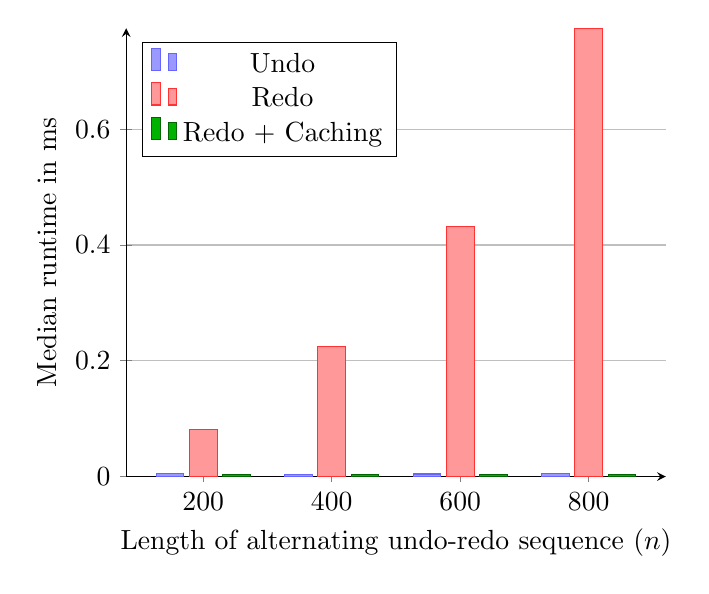
\begin{tikzpicture}
  \begin{axis}[
    ybar,
    ylabel={Median runtime in ms},
    axis y line=left,
    ymin = 0,
    xlabel={Length of alternating undo-redo sequence ($n$)},
    axis x line=bottom,
    symbolic x coords={200, 400, 600, 800},
    ymajorgrids=true,
    yminorgrids=true,
    enlarge x limits = 0.2,
    legend pos = north west,
  ] 

  % undo
  \addplot+[ybar, blue!60, fill=blue!40, postaction={}] coordinates {
  (200, 0.005376994609832764)
  (400, 0.004238009452819824)
  (600, 0.004424989223480225)
  (800, 0.005043983459472656)
  };

  % redo without cache opt
  \addplot+[ybar, red!80, fill=red!40, postaction={}] coordinates {
  (200, 0.08157795667648315)
  (400, 0.22508305311203003)
  (600, 0.43157899379730225)
  (800, 0.7744320034980774)
  }; 

  % redo with cache opt
  \addplot+[ybar, green!40!black, fill=\green, postaction={}] coordinates {
  (200, 0.002785980701446533)
  (400, 0.00341796875)
  (600, 0.003712952136993408)
  (800, 0.004239976406097412)
  };

  \legend{Undo, Redo, Redo + Caching};
  \end{axis} 
  \end{tikzpicture} 
  \end{adjustbox}
  \caption{
    Runtime of resolving the head of a sequence of alternating undo-redo operations of length $n$.
  }\label{fig:runtime-undo-redo-alt}
  \end{figure}
\end{frame}

\begin{frame}[fragile]{Outlook}
  \begin{itemize}
    \item foundation for undo and redo
    \item flexible approach: could mix different undo behaviors
    \pause
    \item open question: how to extend beyond a single register?
  \end{itemize}

  \begin{figure}
    \begin{adjustbox}{max totalsize={\textwidth}{0.75\textheight},center}
    \begin{tikzpicture}[node distance=60pt]
        \node[] (json) at (0,0) {
          \begin{lstlisting}
          {
            *@\colorbox{opset1!10}{A: a,}@*
            *@\colorbox{opset2!10}{B: [b1, b2]}@*
          }
          \end{lstlisting}
        };
  
        \pause
        \node[right=90pt of json,rectangle,draw] (box) {
            Replicated Registers
          };
  
        \draw[-latex,->] (box.west) to [bend right=45] (1.3,0.4);
        \draw[-latex,->] (box.west) to [bend left=55] (1.0,-0.6);
        \draw[-latex,->] (box.west) to [bend left=50] (1.6,-0.6);
        \draw[-latex,->] (box.west) to [bend left=45] (2.3,-0.6);
    \end{tikzpicture}
    \end{adjustbox}
  \end{figure}
\end{frame}

\begin{frame}[standout]
  Questions? Feedback? \\
  \vspace{1.2em}
  \small
  \texttt{
    Reach us at \\
    \href{mailto:lstwn@mailbox.org}{lstwn@mailbox.org} \\
    \href{mailto:martin@kleppmann.com}{martin@kleppmann.com}
  } \\
  \vspace{1.6em}
  
\includegraphics[height=0.44\textheight]{arxiv-qr-code.png}
\end{frame}

\end{document}

% \subsection{Background}

% \begin{frame}[fragile]{Why Replicated Registers, if Automerge is a JSON CRDT?}
%   \begin{figure}
%     \center
%     \includegraphics[height=0.5\textheight]{paper.png}
%   \end{figure}
%   \pause

%   \begin{figure}
%   \begin{adjustbox}{max totalsize={\textwidth}{0.75\textheight},center}
%   \begin{tikzpicture}[node distance=60pt]
%      \node[] (json) at (0,0) {
%         \begin{lstlisting}
%         {
%           *@\colorbox{opset1!10}{A: a,}@*
%           *@\colorbox{opset2!10}{B: [b1, b2]}@*
%         }
%         \end{lstlisting}};

%       \pause
%       \node[right=90pt of json,rectangle,draw] (box) {
%           Replicated Registers
%         };

%       \draw[-latex,->] (box.west) to [bend right=45] (1.3,0.4);

%       \draw[-latex,->] (box.west) to [bend left=55] (1.0,-0.6);
%       \draw[-latex,->] (box.west) to [bend left=50] (1.6,-0.6);
%       \draw[-latex,->] (box.west) to [bend left=45] (2.3,-0.6);
%   \end{tikzpicture}
%   \end{adjustbox}
%   \end{figure}
% \end{frame}

% \subsection{Edge Cases}

% % Undo has to restore conflicts if it undoes a merge operation.
% \setbeamercovered{transparent=35}
% \begin{frame}[fragile]{Edge Cases to Consider (1)}
%   \begin{figure}
%     \begin{adjustbox}{max totalsize={\textwidth}{0.75\textheight},center}
% \begin{tikzpicture}[node distance=60pt]
%   \tikzset{
%     register/.style={
%       anchor=west,
%       xshift=-90pt,
%     },
%   }
%   \def\dist{18pt}

%   \only<1>{
%     \node[register] (vals) at (0, 2) {\textbf{Register: }\stack{
%           \colorbox{black}{\phantom{R}}
%     }};
%   }
%   \only<2,4>{
%     \node[register] (vals) at (0, 2) {\textbf{Register: }\stack{
%           \colorbox{green}{\phantom{R}}, \colorbox{red}{\phantom{R}}
%     }};
%   }
%   \only<3>{
%     \node[register] (vals) at (0, 2) {\textbf{Register: }\stack{
%           \colorbox{blue}{\phantom{R}}
%     }};
%   }

%   % nodes and edges
%   \visible<1->{
%     \node[op] (a1) at (0, 0) {\setop{1}{A}{\colorbox{black}{\phantom{R}}}};
%   }

%   \visible<2->{
%     \node[op,above right=\dist of a1] (a2) {\setop{2}{A}{\colorbox{red}{\phantom{R}}}} edge [pred] (a1);
%     \node[op,below right=\dist of a1] (b2) {\setop{2}{B}{\colorbox{green}{\phantom{R}}}} edge [pred] (a1);
%   }

%   \visible<3->{
%     \node[op,below right=\dist of a2] (a3) {\setop{3}{A}{\colorbox{blue}{\phantom{R}}}} edge [pred] (a2) edge [pred] (b2);
%   }

%   \visible<4->{
%     \node[op,above right=\dist of a3] (a4) {\undop{4}{A}{3}{A}} edge [pred] (a3) edge [anchorref,bend right=30] (a3);
%   }

%   % invisible
%   \node[inv,below right=\dist of a4] (b5) {\phantom{\redop{5}{B}{4}{B}}};
% \end{tikzpicture}
% \end{adjustbox}
% \caption{
%   Undo of a merge op.
% }\label{fig:undo-merge-op}
% \end{figure}
% \end{frame}
% \setbeamercovered{invisible}

% \setbeamercovered{transparent=35}
% \begin{frame}[fragile]{Edge Cases to Consider (2)}
%   \begin{figure}
%     \begin{adjustbox}{max totalsize={\textwidth}{0.75\textheight},center}
% \begin{tikzpicture}[node distance=60pt]
%   \tikzset{
%     register/.style={
%       anchor=west,
%       xshift=-90pt,
%     },
%   }
%   \def\dist{18pt}

%   \only<1->{
%     \node[register] (vals) at (0, 2) {\textbf{Register: }\stack{
%           \colorbox{orange}{\phantom{R}}, \colorbox{green}{\phantom{R}}, \colorbox{red}{\phantom{R}}
%     }};
%   }

%   % nodes and edges
%   \node[op] (a1) at (0, 0) {\setop{1}{A}{\colorbox{black}{\phantom{R}}}};

%   \node[op,above right=\dist of a1] (a2) {\setop{2}{A}{\colorbox{red}{\phantom{R}}}} edge [pred] (a1);
%   \node[op,below right=\dist of a1] (b2) {\setop{2}{B}{\colorbox{green}{\phantom{R}}}} edge [pred] (a1);

%   \node[op,below right=\dist of a2] (a3) {\setop{3}{A}{\colorbox{blue}{\phantom{R}}}} edge [pred] (a2) edge [pred] (b2);

%   \node[op,above right=\dist of a3] (a4) {\undop{4}{A}{3}{A}} edge [pred] (a3) edge [anchorref,bend right=30] (a3);

%   \node[op,below right=\dist of a3] (b4) {\setop{4}{B}{\colorbox{orange}{\phantom{R}}}} edge [pred] (a3);

%   % invisible
%   \node[inv,below right=\dist of a4] (b5) {\phantom{\redop{5}{B}{4}{B}}};
% \end{tikzpicture}
% \end{adjustbox}
% \caption{
%   Concurrent undo and set op.
% }\label{fig:concurrent-undo-set}
% \end{figure}
% \end{frame}
% \setbeamercovered{invisible}

% \setbeamercovered{transparent=35}
% \begin{frame}[fragile]{Edge Cases to Consider (3)}
%   \begin{figure}
%     \begin{adjustbox}{max totalsize={\textwidth}{0.75\textheight},center}
% \begin{tikzpicture}[node distance=60pt]
%   \tikzset{
%     register/.style={
%       anchor=west,
%       xshift=-90pt,
%     },
%   }
%   \def\dist{18pt}

%   \only<1->{
%     \node[register] (vals) at (0, 2) {\textbf{Register: }\stack{
%           \colorbox{black}{\phantom{R}}, \colorbox{green}{\phantom{R}}, \colorbox{red}{\phantom{R}}
%     }};
%   }

%   % nodes and edges
%   \node[op] (a1) at (0, 0) {\setop{1}{A}{\colorbox{black}{\phantom{R}}}};

%   \node[op,above right=\dist of a1] (a2) {\setop{2}{A}{\colorbox{red}{\phantom{R}}}} edge [pred] (a1);
%   \node[op,below right=\dist of a1] (b2) {\setop{2}{B}{\colorbox{green}{\phantom{R}}}} edge [pred] (a1);

%   \node[op,below right=\dist of a2] (a3) {\setop{3}{A}{\colorbox{blue}{\phantom{R}}}} edge [pred] (a2) edge [pred] (b2);

%   \node[op,above right=\dist of a3] (a4) {\undop{4}{A}{3}{A}} edge [pred] (a3) edge [anchorref,bend right=30] (a3);

%   \node[op,below right=\dist of a3] (b4) {\undop{4}{B}{2}{B}} edge [pred] (a3) edge [anchorref,bend left=30] (b2);

%   % invisible
%   \node[inv,below right=\dist of a4] (b5) {\phantom{\redop{5}{B}{4}{B}}};
% \end{tikzpicture}
% \end{adjustbox}
% \caption{
%   Concurrent undo ops.
% }\label{fig:concurrent-undos}
% \end{figure}
% \end{frame}
% \setbeamercovered{invisible}

% \setbeamercovered{transparent=35}
% \begin{frame}[fragile]{Edge Cases to Consider (4)}
%   \begin{figure}
%     \begin{adjustbox}{max totalsize={\textwidth}{0.75\textheight},center}
% \begin{tikzpicture}[node distance=60pt]
%   \tikzset{
%     register/.style={
%       anchor=west,
%       xshift=-90pt,
%     },
%   }
%   \def\dist{18pt}

%   \only<1->{
%     \node[register] (vals) at (0, 2) {\textbf{Register: }\stack{
%           \colorbox{blue}{\phantom{R}}
%     }};
%   }

%   % nodes and edges
%   \node[op] (a1) at (0, 0) {\setop{1}{A}{\colorbox{black}{\phantom{R}}}};

%   \node[op,above right=\dist of a1] (a2) {\setop{2}{A}{\colorbox{red}{\phantom{R}}}} edge [pred] (a1);
%   \node[op,below right=\dist of a1] (b2) {\setop{2}{B}{\colorbox{green}{\phantom{R}}}} edge [pred] (a1);

%   \node[op,below right=\dist of a2] (a3) {\setop{3}{A}{\colorbox{blue}{\phantom{R}}}} edge [pred] (a2) edge [pred] (b2);

%   \node[op,above right=\dist of a3] (a4) {\undop{4}{A}{3}{A}} edge [pred] (a3) edge [anchorref,bend right=30] (a3);

%   \node[op,below right=\dist of a3] (b4) {\undop{4}{B}{2}{B}} edge [pred] (a3) edge [anchorref,bend left=30] (b2);

%   \node[op,below right=\dist of a4] (b5) {\redop{5}{B}{4}{B}} edge [pred] (b4) edge [pred] (a4) edge [anchorref,bend left=30] (b4);
% \end{tikzpicture}
% \end{adjustbox}
% \caption{
%   Redo restores state prior to its corresponding undo.
% }\label{fig:edge-case-3}
% \end{figure}
% \end{frame}
% \setbeamercovered{invisible}

% \subsection{Evaluation}

% \begin{frame}{Constant Runtime for Common Editing Scenarios}
%   \begin{figure}
%   \begin{adjustbox}{max totalsize={\textwidth}{0.75\textheight},center}
%   \begin{tikzpicture}
%   \begin{axis}[
%     xlabel={Length of undo/redo sequence ($n$)},
%     ylabel={Runtime in ms},
%     xmin=0,
%     axis x line=bottom,
%     axis y line=left,
%     ymin=0,
%     ymax=0.010,
%     legend pos=north east,
%     ymajorgrids=true,
%     yticklabel style={
%       /pgf/number format/fixed,
%       /pgf/number format/precision=5
%     },
%     scaled y ticks=false 
%   ]

%   % undo data
%   \addplot[
%     color=blue,
%   ] coordinates {
%   (1, 0.006290340563282371)
%   (2, 0.003907741687726229)
%   (3, 0.002766803983831778)
%   (4, 0.0017496687069069594)
%   (5, 0.0016760083672124892)
%   (6, 0.001955396990524605)
%   (7, 0.001345782628050074)
%   (8, 0.0019154881010763347)
%   (9, 0.0013770495424978435)
%   (10, 0.001276014547329396)
%   (11, 0.0015485882759094238)
%   (12, 0.0013692353677470237)
%   (13, 0.0013271856296341866)
%   (14, 0.0013679209514521062)
%   (15, 0.001304528908804059)
%   (16, 0.0013366359926294535)
%   (17, 0.0013435808941721916)
%   (18, 0.00134780234657228)
%   (19, 0.0014081033586990088)
%   (20, 0.0013913525617681444)
%   (21, 0.0013268127804622054)
%   (22, 0.001440957625163719)
%   (23, 0.0016200695536099374)
%   (24, 0.0016375818522647023)
%   (25, 0.0013710299390368164)
%   (26, 0.0013164350239094347)
%   (27, 0.0014119130210019648)
%   (28, 0.0013253243814688176)
%   (29, 0.0013492428988683969)
%   (30, 0.0013712448126170784)
%   (31, 0.0014037845248822123)
%   (32, 0.0013481056957971305)
%   (33, 0.0013890777481719851)
%   (34, 0.0013086109538562596)
%   (35, 0.001314542896579951)
%   (36, 0.0015176087035797536)
%   (37, 0.0013542969536501914)
%   (38, 0.0013883131032343954)
%   (39, 0.0013373843976296484)
%   (40, 0.0013278163387440145)
%   (41, 0.0013506945979315788)
%   (42, 0.0016484785883221775)
%   (43, 0.0013150325394235551)
%   (44, 0.0013713290682062507)
%   (45, 0.0012379433319438249)
%   (46, 0.0012963268964085728)
%   (47, 0.0012237174669280648)
%   (48, 0.0012681810767389834)
%   (49, 0.001609297381946817)
%   (50, 0.0013969987630844116)
%   };

%   % redo data
%   \addplot[
%     color=red,
%   ] coordinates {
%   (1, 0.007437939144438133)
%   (2, 0.003633987420471385)
%   (3, 0.002511455590138212)
%   (4, 0.0022350119543261826)
%   (5, 0.0018720132065936923)
%   (6, 0.0019328816561028361)
%   (7, 0.00187860953155905)
%   (8, 0.002103224309394136)
%   (9, 0.0023768509563524276)
%   (10, 0.001951182057382539)
%   (11, 0.0027914689562749118)
%   (12, 0.002302225591847673)
%   (13, 0.0018702853412833065)
%   (14, 0.001864643389126286)
%   (15, 0.0019206689321435988)
%   (16, 0.0019472866551950574)
%   (17, 0.0018687470292206854)
%   (18, 0.0019792676030192524)
%   (19, 0.002029231225606054)
%   (20, 0.001964766182936728)
%   (21, 0.0019252107886131853)
%   (22, 0.0018749097071122378)
%   (23, 0.001866210310254246)
%   (24, 0.0018289572326466441)
%   (25, 0.0021713866444770247)
%   (26, 0.002587106981081888)
%   (27, 0.0018908421625383198)
%   (28, 0.0018309024162590504)
%   (29, 0.0019520004279911518)
%   (30, 0.002062761748675257)
%   (31, 0.001968364085769281)
%   (32, 0.002528973447624594)
%   (33, 0.002954049239633605)
%   (34, 0.0026645801845006645)
%   (35, 0.002441259188344702)
%   (36, 0.002502664952771738)
%   (37, 0.002708020620048046)
%   (38, 0.002156659436877817)
%   (39, 0.0021457494294736534)
%   (40, 0.0019089243141934276)
%   (41, 0.0019161189266014844)
%   (42, 0.0019302570726722479)
%   (43, 0.004374536831164733)
%   (44, 0.0019373227842152119)
%   (45, 0.0017444676195736974)
%   (46, 0.0018851725617423654)
%   (47, 0.001839210162870586)
%   (48, 0.0020025315461680293)
%   (49, 0.0019971978035755455)
%   (50, 0.002073564799502492)
%   };

%   \legend{Undo, Redo}

%   \end{axis}
%   \end{tikzpicture}
%   \end{adjustbox}
%   \caption{
%     Runtime of the last undo/redo operation in a sequence
%     of $n$ consecutive undo/redo operations.
%   }\label{fig:runtime-cons-undo-redo}
%   \end{figure}
% \end{frame}

% \begin{frame}[standout]
%   Questions? Feedback? \\
%   \vspace{1.2em}
%   \small
%   \texttt{
%     Reach us at \\
%     \href{mailto:lstwn@mailbox.org}{lstwn@mailbox.org} \\
%     \href{mailto:martin@kleppmann.com}{martin@kleppmann.com}
%   } \\
%   \vspace{1.2em}
%   \includegraphics[height=0.4\textheight]{qrcode_undo_paper.png}
% \end{frame}
% \setbeamercovered{invisible}

% \appendix{}

% \begin{frame}[allowframebreaks]
%     \printbibliography{}
% \end{frame}

% \section*{Backup Slides}

% \subsection{Extended Semantics}

% \begin{frame}[fragile]
%   \begin{figure}
%     \begin{adjustbox}{max totalsize={\textwidth}{0.75\textheight},center}
%       \begin{tikzpicture}[node distance=0.23cm]
%         \coordinate (c1) at (0,0);

%         \tikzset{
%           canvas/.style={
%             rectangle,
%             draw,
%             anchor = west,
%             inner sep = 4pt,
%           },
%           rect/.style={
%             rectangle,
%             minimum width = 1.2cm, 
%             minimum height = 0.5cm,
%             inner sep = 0.1cm,
%             text = white,
%             fill = #1,
%           },
%           optrans/.style={
%             <-,bend right=90,>={Stealth[round]},
%             swap,
%             black!70,
%           },
%           casediv/.style={
%             black!70,
%           },
%         }

%         \def\black{black}
%         \def\green{green!60!black}
%         \def\red{red}
%         \def\upperoffset{20pt}
%         \def\loweroffset{50pt}

%         \onslide<1->{
%         \node[
%           canvas,
%           label={[]above:(1a)},
%         ] (1a) at (c1) {
%           \begin{tikzpicture}[node distance=3pt]
%             \node[
%                 rect=\black,
%               ] (r1) at (0,0) {\vphantom{bg}black};
%             \node[
%                 rect=\black,
%                 below = of r1,
%               ] (r2) {\vphantom{bg}black};
%           \end{tikzpicture}
%         };
%         }

%         \onslide<3->{
%         \node[
%           canvas,
%           label={[]above:(1b)},
%           right = of 1a,
%         ] (1b) {
%           \begin{tikzpicture}[node distance=3pt]
%             \node[
%                 rect=\red,
%               ] (r1) at (0,0) {\vphantom{bg}red};
%             \node[
%                 rect=\black,
%                 below = of r1,
%               ] (r2) {\vphantom{bg}black};
%           \end{tikzpicture}
%         } edge (1a);
%         }

%         \onslide<5->{
%         \node[
%           canvas,
%           label={[]above:(1c)},
%           right = of 1b,
%         ] (1c) {
%           \begin{tikzpicture}[node distance=3pt]
%             \node[
%                 rect=\red,
%               ] (r1) at (0,0) {\vphantom{bg}red};
%             \node[
%                 rect=\green,
%                 below = of r1,
%               ] (r2) {\vphantom{bg}green};
%           \end{tikzpicture}
%         } edge (1b);
%         }

%         \onslide<7->{
%         \node[
%           canvas,
%           label={[]above:(1d)},
%           right = of 1c,
%         ] (1d) {
%           \begin{tikzpicture}[node distance=3pt]
%             \node[
%                 rect=\black,
%               ] (r1) at (0,0) {\vphantom{bg}black};
%             \node[
%                 rect=\green,
%                 below = of r1,
%               ] (r2) {\vphantom{bg}green};
%           \end{tikzpicture}
%         } edge (1c);
%         }

%         \onslide<9->{
%         \node[
%           canvas,
%           label={[]above:(1e)},
%           right = of 1d,
%         ] (1e) {
%           \begin{tikzpicture}[node distance=3pt]
%             \node[
%                 rect=\red,
%               ] (r1) at (0,0) {\vphantom{bg}red};
%             \node[
%                 rect=\green,
%                 below = of r1,
%               ] (r2) {\vphantom{bg}green};
%           \end{tikzpicture}
%         } edge (1d);
%         }

%         \coordinate (d1s) at ($(1a.north)!0.5!(1b.north)+(0,+\upperoffset)$);
%         \coordinate (d1e) at ($(1a.north)!0.5!(1b.north)+(0,-\loweroffset)$);

%         \coordinate (d2s) at ($(1b.north)!0.5!(1c.north)+(0,+\upperoffset)$);
%         \coordinate (d2e) at ($(1b.north)!0.5!(1c.north)+(0,-\loweroffset)$);

%         \coordinate (d3s) at ($(1c.north)!0.5!(1d.north)+(0,+\upperoffset)$);
%         \coordinate (d3e) at ($(1c.north)!0.5!(1d.north)+(0,-\loweroffset)$);

%         \coordinate (d4s) at ($(1d.north)!0.5!(1e.north)+(0,+\upperoffset)$);
%         \coordinate (d4e) at ($(1d.north)!0.5!(1e.north)+(0,-\loweroffset)$);

%         \onslide<2->{
%         \draw[stepline] (d1s) -- (d1e);
%         \draw (1b.north)+(-0.2cm,+\upperoffset) edge ["A set",optrans] ($(1a.north)+(0,+\upperoffset)$);
%         }

%         \onslide<4->{
%         \draw (1c.north)+(-0.2cm,+\upperoffset) edge ["B set",optrans] ($(1b.north)+(0,+\upperoffset)$);
%         \draw[stepline] (d2s) -- (d2e);
%         }

%         \onslide<6->{
%         \draw (1d.north)+(-0.2cm,+\upperoffset) edge ["A undo",optrans] ($(1c.north)+(0,+\upperoffset)$);
%         \draw[stepline] (d3s) -- (d3e);
%         }

%         \onslide<8->{
%         \draw (1e.north)+(-0.2cm,+\upperoffset) edge ["A redo",optrans] ($(1d.north)+(0,+\upperoffset)$);
%         \draw[stepline] (d4s) -- (d4e);
%         }

%       \end{tikzpicture}
%     \end{adjustbox}
%     \caption{Canvas with two replicated registers.}\label{fig:intro-two-registers}
%   \end{figure}
% \end{frame}

% \begin{frame}[fragile]
%   \begin{figure}
%     \begin{adjustbox}{max totalsize={\textwidth}{0.75\textheight},center}
%       \begin{tikzpicture}[node distance=0.23cm]
%         \coordinate (c1) at (0,-1.6);

%         \tikzset{
%           canvas/.style={
%             rectangle,
%             draw,
%             anchor = west,
%             inner sep = 4pt,
%           },
%           rect/.style={
%             rectangle,
%             minimum width = 1.2cm, 
%             minimum height = 0.5cm,
%             inner sep = 0.1cm,
%             text = white,
%             fill = #1,
%           },
%           optrans/.style={
%             <-,bend right=90,>={Stealth[round]},
%             swap,
%             black!70,
%           },
%           casediv/.style={
%             black!70,
%           },
%         }

%         \def\black{black}
%         \def\green{green!60!black}
%         \def\red{red}
%         \def\upperoffset{20pt}
%         \def\loweroffset{120pt}

%         \coordinate (d1s) at ($(1a.north)!0.5!(1b.north)+(0,+\upperoffset)$);
%         \coordinate (d1e) at ($(1a.north)!0.5!(1b.north)+(0,-\loweroffset)$);

%         \coordinate (d2s) at ($(1b.north)!0.5!(1c.north)+(0,+\upperoffset)$);
%         \coordinate (d2e) at ($(1b.north)!0.5!(1c.north)+(0,-\loweroffset)$);

%         \coordinate (d3s) at ($(1c.north)!0.5!(1d.north)+(0,+\upperoffset)$);
%         \coordinate (d3e) at ($(1c.north)!0.5!(1d.north)+(0,-\loweroffset)$);

%         \coordinate (d4s) at ($(1d.north)!0.5!(1e.north)+(0,+\upperoffset)$);
%         \coordinate (d4e) at ($(1d.north)!0.5!(1e.north)+(0,-\loweroffset)$);

%         \onslide<2->{
%         \draw (1b.north)+(-0.2cm,+\upperoffset) edge ["A set",optrans] ($(1a.north)+(0,+\upperoffset)$);
%         \draw[stepline] (d1s) -- (d1e);
%         }

%         \onslide<4->{
%         \draw (1c.north)+(-0.2cm,+\upperoffset) edge ["B set",optrans] ($(1b.north)+(0,+\upperoffset)$);
%         \draw[stepline] (d2s) -- (d2e);
%         }

%         \onslide<6->{
%         \draw (1d.north)+(-0.2cm,+\upperoffset) edge ["A undo",optrans] ($(1c.north)+(0,+\upperoffset)$);
%         \draw[stepline] (d3s) -- (d3e);
%         }

%         \onslide<9->{
%         \draw (1e.north)+(-0.2cm,+\upperoffset) edge ["A redo",optrans] ($(1d.north)+(0,+\upperoffset)$);
%         \draw[stepline] (d4s) -- (d4e);
%         }

%         %%%%
        
%         \onslide<1->{
%         \node[
%           canvas,
%           label={[]above:(2a)},
%         ] (2a) at (c1) {
%           \begin{tikzpicture}[node distance=3pt]
%             \node[
%                 rect=\black,
%               ] (r1) at (0,0) {\vphantom{bg}black};
%           \end{tikzpicture}
%         };
%         }

%         \onslide<3->{
%         \node[
%           canvas,
%           label={[]above:(2b)},
%           right = of 2a,
%         ] (2b) {
%           \begin{tikzpicture}[node distance=3pt]
%             \node[
%                 rect=\red,
%               ] (r1) at (0,0) {\vphantom{bg}red};
%           \end{tikzpicture}
%         } edge (2a);
%         }

%         \onslide<5->{
%         \node[
%           canvas,
%           label={[]above:(2c)},
%           right = of 2b,
%         ] (2c) {
%           \begin{tikzpicture}[node distance=3pt]
%             \node[
%                 rect=\green,
%               ] (r1) at (0,0) {\vphantom{bg}green};
%           \end{tikzpicture}
%         } edge (2b);
%         }

%         %%%

%         \onslide<8->{
%         \node[
%           canvas,
%           label={[]above:(2d1)},
%           above right = of 2c,
%           xshift=+2pt,
%           yshift=+4pt,
%         ] (2d1) {
%           \begin{tikzpicture}[node distance=3pt]
%             \node[
%                 rect=\black,
%               ] (r1) at (0,0) {\vphantom{bg}black};
%           \end{tikzpicture}
%         } edge (2c);
%         }

%         \onslide<11->{
%         \node[
%           canvas,
%           label={[]above:(2e1)},
%           above right = of 2d1,
%           xshift=+2pt,
%           yshift=-7pt,
%         ] (2d1e1) {
%           \begin{tikzpicture}[node distance=3pt]
%             \node[
%                 rect=\red,
%               ] (r1) at (0,0) {\vphantom{bg}red};
%           \end{tikzpicture}
%         } edge (2d1);
%         }

%         \onslide<11->{
%         \node[
%           canvas,
%           label={[]above:(2e2)},
%           below right = of 2d1,
%           xshift=+2pt,
%           yshift=+7pt,
%         ] (2d1e2) {
%           \begin{tikzpicture}[node distance=3pt]
%             \node[
%                 rect=\green,
%               ] (r1) at (0,0) {\vphantom{bg}green};
%           \end{tikzpicture}
%         } edge (2d1);
%         }

%         %%%

%         \onslide<7->{
%         \node[
%           canvas,
%           label={[]above:(2d2)},
%           below right = of 2c,
%           xshift=+2pt,
%           yshift=-4pt,
%         ] (2d2) {
%           \begin{tikzpicture}[node distance=3pt]
%             \node[
%                 rect=\red,
%               ] (r1) at (0,0) {\vphantom{bg}red};
%           \end{tikzpicture}
%         } edge (2c);
%         }

%         \onslide<10->{
%         \node[
%           canvas,
%           label={[]above:(2e3)},
%           right = of 2d2,
%         ] (2e2) {
%           \begin{tikzpicture}[node distance=3pt]
%             \node[
%                 rect=\green,
%               ] (r1) at (0,0) {\vphantom{bg}green};
%           \end{tikzpicture}
%         } edge (2d2);
%         }

%       \end{tikzpicture}
%     \end{adjustbox}
%     \caption{Canvas with one replicated register.}\label{fig:intro-one-register}
%   \end{figure}
% \end{frame}

% \setbeamercovered{transparent}
% \begin{frame}[fragile]
%   \begin{figure}
%     \begin{adjustbox}{max totalsize={\textwidth}{0.75\textheight},center}
%       \begin{tikzpicture}[node distance=0.23cm]
%         \coordinate (c1) at (0,-1.6);

%         \tikzset{
%           canvas/.style={
%             rectangle,
%             draw,
%             anchor = west,
%             inner sep = 4pt,
%           },
%           rect/.style={
%             rectangle,
%             minimum width = 1.2cm, 
%             minimum height = 0.5cm,
%             inner sep = 0.1cm,
%             text = white,
%             fill = #1,
%           },
%           optrans/.style={
%             <-,bend right=90,>={Stealth[round]},
%             swap,
%             black!70,
%           },
%           casediv/.style={
%             black!70,
%           },
%         }

%         \def\black{black}
%         \def\green{green!60!black}
%         \def\red{red}
%         \def\upperoffset{20pt}
%         \def\loweroffset{120pt}

%         \coordinate (d1s) at ($(1a.north)!0.5!(1b.north)+(0,+\upperoffset)$);
%         \coordinate (d1e) at ($(1a.north)!0.5!(1b.north)+(0,-\loweroffset)$);

%         \coordinate (d2s) at ($(1b.north)!0.5!(1c.north)+(0,+\upperoffset)$);
%         \coordinate (d2e) at ($(1b.north)!0.5!(1c.north)+(0,-\loweroffset)$);

%         \coordinate (d3s) at ($(1c.north)!0.5!(1d.north)+(0,+\upperoffset)$);
%         \coordinate (d3e) at ($(1c.north)!0.5!(1d.north)+(0,-\loweroffset)$);

%         \coordinate (d4s) at ($(1d.north)!0.5!(1e.north)+(0,+\upperoffset)$);
%         \coordinate (d4e) at ($(1d.north)!0.5!(1e.north)+(0,-\loweroffset)$);

%         \draw (1b.north)+(-0.2cm,+\upperoffset) edge ["A set",optrans] ($(1a.north)+(0,+\upperoffset)$);
%         \draw[stepline] (d1s) -- (d1e);

%         \draw (1c.north)+(-0.2cm,+\upperoffset) edge ["B set",optrans] ($(1b.north)+(0,+\upperoffset)$);
%         \draw[stepline] (d2s) -- (d2e);

%         \draw (1d.north)+(-0.2cm,+\upperoffset) edge ["A undo",optrans] ($(1c.north)+(0,+\upperoffset)$);
%         \draw[stepline] (d3s) -- (d3e);

%         \draw (1e.north)+(-0.2cm,+\upperoffset) edge ["A redo",optrans] ($(1d.north)+(0,+\upperoffset)$);
%         \draw[stepline] (d4s) -- (d4e);

%         %%%%
        
%         \onslide<1-2>{
%         \node[
%           canvas,
%           label={[]above:(2a)},
%         ] (2a) at (c1) {
%           \begin{tikzpicture}[node distance=3pt]
%             \node[
%                 rect=\black,
%               ] (r1) at (0,0) {\vphantom{bg}black};
%           \end{tikzpicture}
%         };

%         \node[
%           canvas,
%           label={[]above:(2b)},
%           right = of 2a,
%         ] (2b) {
%           \begin{tikzpicture}[node distance=3pt]
%             \node[
%                 rect=\red,
%               ] (r1) at (0,0) {\vphantom{bg}red};
%           \end{tikzpicture}
%         } edge (2a);

%         \node[
%           canvas,
%           label={[]above:(2c)},
%           right = of 2b,
%         ] (2c) {
%           \begin{tikzpicture}[node distance=3pt]
%             \node[
%                 rect=\green,
%               ] (r1) at (0,0) {\vphantom{bg}green};
%           \end{tikzpicture}
%         } edge (2b);

%         %%%

%         \node[
%           canvas,
%           label={[]above:(2d1)},
%           above right = of 2c,
%           xshift=+2pt,
%           yshift=+4pt,
%         ] (2d1) {
%           \begin{tikzpicture}[node distance=3pt]
%             \node[
%                 rect=\black,
%               ] (r1) at (0,0) {\vphantom{bg}black};
%           \end{tikzpicture}
%         } edge (2c);
%         }

%         \onslide<1>{
%         \node[
%           canvas,
%           label={[]above:(2e1)},
%           above right = of 2d1,
%           xshift=+2pt,
%           yshift=-7pt,
%         ] (2d1e1) {
%           \begin{tikzpicture}[node distance=3pt]
%             \node[
%                 rect=\red,
%               ] (r1) at (0,0) {\vphantom{bg}red};
%           \end{tikzpicture}
%         } edge (2d1);
%         }

%         \onslide<1-2>{
%         \node[
%           canvas,
%           label={[]above:(2e2)},
%           below right = of 2d1,
%           xshift=+2pt,
%           yshift=+7pt,
%         ] (2d1e2) {
%           \begin{tikzpicture}[node distance=3pt]
%             \node[
%                 rect=\green,
%               ] (r1) at (0,0) {\vphantom{bg}green};
%           \end{tikzpicture}
%         } edge (2d1);
%         }

%         %%%

%         \onslide<1>{
%         \node[
%           canvas,
%           label={[]above:(2d2)},
%           below right = of 2c,
%           xshift=+2pt,
%           yshift=-4pt,
%         ] (2d2) {
%           \begin{tikzpicture}[node distance=3pt]
%             \node[
%                 rect=\red,
%               ] (r1) at (0,0) {\vphantom{bg}red};
%           \end{tikzpicture}
%         } edge (2c);

%         \node[
%           canvas,
%           label={[]above:(2e3)},
%           right = of 2d2,
%         ] (2e2) {
%           \begin{tikzpicture}[node distance=3pt]
%             \node[
%                 rect=\green,
%               ] (r1) at (0,0) {\vphantom{bg}green};
%           \end{tikzpicture}
%         } edge (2d2);
%         }

%       \end{tikzpicture}
%     \end{adjustbox}
%     \caption{Canvas with one replicated register.}\label{fig:intro-one-register-chosen-path}
%   \end{figure}
% \end{frame}

% \subsection{Global vs Local Undo}

% \setbeamercovered{transparent=35}
% \begin{frame}[fragile]{Illustration}
%   \begin{figure}
%     \begin{adjustbox}{max totalsize={\textwidth}{0.75\textheight},center}
% \begin{tikzpicture}[node distance=18pt]
%   \tikzset{
%     register/.style={
%       anchor=west,
%       xshift=-30pt,
%     },
%   }
%   \def\dist{18pt}

%   \only<1>{
%     \node[register] (vals) at (0, 2) {\textbf{Register: }\stack{
%       \colorbox{black}{\phantom{R}}
%     }};
%   }
%   \only<2>{
%     \node[register] (vals) at (0, 2) {\textbf{Register: }\stack{
%       \colorbox{red}{\phantom{R}}
%     }};
%   }
%   \only<3>{
%     \node[register] (vals) at (0, 2) {\textbf{Register: }\stack{
%       \colorbox{green}{\phantom{R}}
%     }};
%   }
%   \only<4>{
%     \node[register] (vals) at (0, 2) {\textbf{Register: }\stack{
%       \colorbox{red}{\phantom{R}}
%     }};
%   }
%   \only<5->{
%     \node[register] (vals) at (0, 2) {\textbf{Register: }\stack{
%       \colorbox{black}{\phantom{R}}
%     }};
%   }

%   % nodes and edges
%   \visible<1->{
%     \node[op] (a1) at (0, 0) {\setop{1}{A}{\colorbox{black}{\phantom{R}}}};
%   }

%   \visible<2->{
%     \node[op,right=of a1] (a2) {\setop{2}{A}{\colorbox{red}{\phantom{R}}}} edge [pred] (a1);
%   }

%   \visible<3->{
%     \node[op,right=of a2] (b3) {\setop{3}{B}{\colorbox{green}{\phantom{R}}}} edge [pred] (a2);
%   }

%   \visible<4>{
%     \node[op,right=of b3] (a4_global) {\undop{4}{A}{3}{B}} edge [pred] (b3) edge [anchorref,bend left,label={[anchor=north,font=\footnotesize]below:global undo}] (b3);
%   }

%   \visible<5->{
%     \node[op,right=of b3] (a4_local) {\undop{4}{A}{2}{A}} edge [pred] (b3) edge [anchorref,bend right=50,label={[font=\footnotesize]local undo}] (a2);
%   }

% \end{tikzpicture}
% \end{adjustbox}
% \caption{
%   Local vs global undo.
% }\label{fig:local-vs-global-undo}
% \end{figure}
% \end{frame}
% \setbeamercovered{invisible}

% \subsection{Algorithm}

% \setbeamercovered{transparent=35}
% \begin{frame}[fragile,label=undoalg]
%   \begin{figure}
%     \begin{adjustbox}{max totalsize={\textwidth}{0.75\textheight},center}
% \begin{tikzpicture}[node distance=60pt]
%   \tikzset{
%     register/.style={
%       anchor=west,
%       xshift=-25pt,
%     },
%   }
%   \def\dist{18pt}

%   \only<1>{
%   \node[register] (vals) at (0, 2) {\textbf{Register: }\stack{1}};
%   }
%   \only<2>{
%   \node[register] (vals) at (0, 2) {\textbf{Register: }\stack{2}};
%   }
%   \only<3>{
%   \node[register] (vals) at (0, 2) {\textbf{Register: }\stack{3,4}};
%   }
%   \only<4>{
%   \node[register] (vals) at (0, 2) {\textbf{Register: }\stack{5}};
%   }
%   \only<5>{
%   \node[register] (vals) at (0, 2) {\textbf{Register: }\stack{2}};
%   }
%   \only<6>{
%   \node[register] (vals) at (0, 2) {\textbf{Register: }\stack{3,4,2}};
%   }
%   \only<7>{
%   \node[register] (vals) at (0, 2) {\textbf{Register: }\stack{2}};
%   }
%   \only<8>{
%   \node[register] (vals) at (0, 2) {\textbf{Register: }\stack{6}};
%   }
%   \only<9>{
%   \node[register] (vals) at (0, 2) {\textbf{Register: }\stack{1,6}};
%   }
%   \only<10>{
%   \node[register] (vals) at (0, 2) {\textbf{Register: }\stack{2}};
%   }
%   \only<11>{
%   \node[register] (vals) at (0, 2) {\textbf{Register: }\stack{3,4,2}};
%   }
%   \only<12>{
%   \node[register] (vals) at (0, 2) {\textbf{Register: }\stack{5}};
%   }

%   % nodes and edges
%   \onslide<1,9>{
%   \node[op] (a1) at (0, 0) {\setop{1}{A}{1}};
%   }
%   \visible<2->{
%   \onslide<2,5-6,7,9,10,11>{
%   \node[op,right of=a1] (b2) {\setop{2}{B}{2}} edge [pred] (a1);
%   }
%   }

%   \visible<3->{
%   \onslide<3,5-6,11>{
%   \node[op,above right=\dist of b2] (a3) {\setop{3}{A}{4}} edge [pred] (b2);
%   }
%   }
%   \visible<3->{
%   \onslide<3,6,7,10,11>{
%   \node[op,below right=\dist of b2] (b3) {\setop{3}{B}{3}} edge [pred] (b2);
%   }
%   }

%   \visible<4->{
%   \onslide<4,6,11,12>{
%   \node[op,below right=\dist of a3] (b4) {\setop{4}{B}{5}} edge [pred] (b3) edge [pred] (a3);
%   }
%   }

%   \visible<5->{
%   \onslide<5-6,11>{
%   \node[op,above right=\dist of b4] (a5) {\undop{5}{A}{3}{A}} edge [pred] (b4) edge [anchorref] (a3);
%   }}
%   \visible<6->{
%   \onslide<6,11,12>{
%   \node[op,below right=\dist of b4] (b5) {\undop{5}{B}{4}{B}} edge [pred] (b4) edge [anchorref,bend left] (b4);
%   }}

%   \visible<7->{
%   \onslide<7,10,11>{
%   \node[op,below right=\dist of a5] (b6) {\undop{6}{B}{3}{B}} edge [pred] (b5) edge [pred] (a5) edge [anchorref] (b3);
%   }}

%   \visible<8->{
%   \onslide<8-9>{
%   \node[op,above right=\dist of b6] (a7) {\setop{7}{A}{6}} edge [pred] (b6);
%   }}

%   \begin{scope}[on background layer]
%   \visible<9->{
%   \onslide<9,10>{
%   \node[op,below right=\dist of b6] (b7) {\undop{7}{B}{2}{B}} edge [pred] (b6) edge [anchorref] (b2);
%   }}
%   \end{scope}

%   \visible<10->{
%   \onslide<10>{
%   \node[op,below right=\dist of a7] (b8) {\redop{8}{B}{7}{B}} edge [pred] (b7) edge [pred] (a7) edge [anchorref,bend left] (b7);
%   }}

%   \visible<11->{
%   \onslide<11>{
%   \node[op,right of=b8] (b9) {\redop{9}{B}{6}{B}} edge [pred] (b8) edge [anchorref,bend right=30] (b6);
%   }}

%   \visible<12->{
%   \onslide<12>{
%   \node[op,right of=b9] (b10) {\redop{10}{B}{5}{B}} edge [pred] (b9) edge [anchorref,bend left=35] (b5);
%   }}

% \end{tikzpicture}
% \end{adjustbox}
% \caption{
%   An operation history of a single register with undo and redo\only<11>{
%   \hyperlink{undoalg<6>}{(to undo)}}\only<6>{
%   \hyperlink{undoalg<11>}{(backlink)}}.
% }\label{fig:op-hist-undo-redo}
% \end{figure}
% \end{frame}
% \setbeamercovered{invisible}

% \subsection{Extended Evaluation}

% \setbeamercovered{invisible}
% \begin{frame}[fragile]{Degenerate Editing Scenario}
%   \begin{figure}
%     \begin{adjustbox}{max totalsize={\textwidth}{0.75\textheight},center}
%       \begin{tikzpicture}[node distance=60pt]

%         \node[op] (a1) at (0, 0) {\setop{1}{A}{1}};
%         \pause
%         \node[op,right of=a1] (a2) {\undop{2}{A}{1}{A}} edge [pred] (a1) edge [anchorref,bend left] (a1);
%         \node[op,right of=a2] (a3) {\redop{3}{A}{2}{A}} edge [pred] (a2) edge [anchorref,bend left] (a2);
%         \pause
%         \node[op,right of=a3] (a4) {\undop{4}{A}{1}{A}} edge [pred] (a3) edge [anchorref,bend right=45] (a1);
%         \node[op,right of=a4] (a5) {\redop{5}{A}{4}{A}} edge [pred] (a4) edge [anchorref,bend left] (a4);
%         \pause
%         \node[op,right of=a5] (a6) {\undop{6}{A}{1}{A}} edge [pred] (a5) edge [anchorref,bend right=55] (a1);
%         \node[head,right of=a6] (a7) {\redop{7}{A}{6}{A}} edge [pred] (a6) edge [anchorref,bend left] (a6);

%       \end{tikzpicture}
%     \end{adjustbox}
%     \caption{Sequence of alternating undo-redo operations\only<1>{.}
%     \only<2->{of length }\only<2>{1}\only<3>{2}\only<4>{3}\only<2->{.}
%     }\label{fig:degenerate-editing-scenario}
%   \end{figure}
% \end{frame}

% \begin{frame}{Linear Runtime for Impractical Scenarios}
%   \begin{figure}
%     \begin{adjustbox}{max totalsize={\textwidth}{0.75\textheight},center}
%       \begin{tikzpicture}
%       \begin{axis}[
%         ybar,
%         ylabel={Runtime in ms},
%         axis y line=left,
%         ymin = 0,
%         xlabel={Length of alternating undo-redo sequence ($n$)},
%         axis x line=bottom,
%         symbolic x coords={200, 400, 600, 800},
%         ymajorgrids=true,
%         yminorgrids=true,
%         enlarge x limits = 0.2,
%         legend pos = north west,
%       ] 

%       % undo
%       \addplot+ coordinates {
%       (200, 0.00504857866326347)
%       (400, 0.005509669485036284)
%       (600, 0.006512108666356653)
%       (800, 0.007120864116586745)
%       };

%       % redo
%       \addplot+ coordinates {
%       (200, 0.11390662190387957)
%       (400, 0.3034253417572472)
%       (600, 0.5630059454997536)
%       (800, 0.9230491668859031)
%       }; 

%       \legend{Undo, Redo};
%       \end{axis} 
%       \end{tikzpicture} 
%     \end{adjustbox}
%     \caption{
%     Runtime of the last undo/redo operation
%     in a sequence of alternating undo-redo operations of length $n$.
%     }\label{fig:runtime-undo-redo-alt}
%   \end{figure}
% \end{frame}

% \subsection{Undo Taxonomy}

% \begin{frame}{A Taxonomy of Undo Behavior}
%   \begin{table}
%     \centering
%     \begin{tabular}{@{}ccc@{}}
%             Order $\backslash$ Origin
%             & \makecell{Generating\\Replica}
%             & \makecell{Any\\Replica}
%             \\
%         \midrule
%             \makecell{Reverse\\ Chronological}
%             & \alert{local undo}
%             & global undo
%             \\
%         \midrule
%             Selective
%             & \multicolumn{2}{c}{revert\footnote{often called \emph{selective undo} in the literature~\cite{Yu2015undo}}}
%             \\
%     \end{tabular}
%   \end{table}
% \end{frame}

% \begin{frame}[fragile]{Undo Kinds in a Collaborative Setting}
%   \begin{figure}
%     \center
%     \begin{adjustbox}{max totalsize={\textwidth}{0.75\textheight},center}
%         \tikzset{
%           treenode/.style = {shape=rectangle, rounded corners,
%                              draw, align=center,},
%           root/.style     = {treenode},
%           dummy/.style    = {circle,draw}
%         }
%         \begin{tikzpicture}
%           [
%             grow                    = right,
%             sibling distance        = 6em,
%             level distance          = 10em,
%             edge from parent/.style = {draw, -latex},
%             every node/.style       = {font=\footnotesize},
%             sloped
%           ]
%           \node [root,dummy] {}
%             child { node [treenode, align=center] {selective undo}
%               edge from parent node [below] {any order} }
%             child { node [treenode] {undo}
%               child { node [treenode] {global undo}
%                 edge from parent node [below] {all ops} }
%               child { node [treenode] {local undo}
%                 edge from parent node [above, align=center] {own ops} }
%               edge from parent node [above, align=center] {rev. chron. order} };
%         \end{tikzpicture}
%       \end{adjustbox}
%   \end{figure}
% \end{frame}
